\chapter{\texorpdfstring{More BPMN}{More BPMN}}
\label{ch:07b}
\lecturemeta{Lezione 07b \quad\textbullet\quad 2026-07-03 \quad\textbullet\quad Roberto Bruni}{Weske, \emph{Business Process Management}, Sect.4.3, 4.7, 5.7 · Dumas et al., \emph{Fundamentals of BPM}, Ch.3-4}

In \hyperref[ch:07a]{07a — EPC e BPMN} abbiamo visto lo scheletro di BPMN — swimlane, flow objects, connecting objects. Questa lezione aggiunge gli elementi che rendono BPMN davvero espressivo (e complesso): gli \textbf{artefact} (dati, gruppi, annotazioni), i \textbf{marker} che specializzano attività ed eventi, la ricchezza degli \textbf{eventi} catching/throwing, la modellazione della comunicazione con \textbf{collaboration} e \textbf{message flow}, il riuso tramite \textbf{call activity}, e infine le \textbf{choreography} con la loro notazione a bande.

\section{\texorpdfstring{Artefact e associazioni}{Artefact e associazioni}}

Oltre agli elementi che influenzano il flusso, BPMN permette di aggiungere informazione "di contorno" tramite gli \textbf{artefact}. Sono pensati per dare flessibilità: un tool può estendere la notazione base aggiungendo artefact adatti al dominio. Ne esistono tre tipi predefiniti — \textbf{data object}, \textbf{group} e \textbf{text annotation} — ma la caratteristica comune è che \textbf{non hanno effetto diretto} sul sequence flow o sul message flow: servono solo a documentare.

Gli artefact si collegano agli oggetti del flusso tramite un'\textbf{association}, rappresentata da una linea punteggiata (con eventuale punta). La \textbf{text annotation}, in particolare, è un commento a fumetto (call-out punteggiato) che si aggancia a qualsiasi oggetto per fornire documentazione aggiuntiva. Il \textbf{group} (rettangolo arrotondato a linee tratteggiate) raggruppa oggetti che logicamente stanno insieme, sempre \textbf{senza effetto comportamentale}.

\section{\texorpdfstring{Marker: specializzare attività ed eventi}{Marker: specializzare attività ed eventi}}

La filosofia di BPMN, ricordiamo, è "poche forme base, tanti marker". I \textbf{marker} interni di un'attività dicono due cose: la sua \textbf{natura} (il \emph{task type}) e il \textbf{modo in cui viene eseguita} (l'\emph{activity marker}).

\begin{boxdefinition}{Task type (la natura dell'attività)}
\begin{itemize}
\item \textbf{Send / Receive task}: inviano o ricevono un messaggio.
\item \textbf{User task}: richiede l'interazione diretta di una persona \emph{attraverso un'interfaccia}, con l'aiuto di un sistema software.
\item \textbf{Manual task}: eseguita \emph{interamente} da una persona, \textbf{senza} l'assistenza di un computer.
\item \textbf{Service task}: task automatico in cui il processo interagisce con un \textbf{servizio/sistema esterno} (web service, API), senza intervento umano.
\item \textbf{Script task}: task automatico in cui uno \textbf{script} (JavaScript, Python, ...) è eseguito \textbf{internamente} al motore BPMN, senza chiamare servizi esterni.
\item \textbf{Business rule task}: valuta un insieme di regole di business.
\end{itemize}
\end{boxdefinition}

\begin{boxdefinition}{Activity marker (il modo di esecuzione)}
\begin{itemize}
\item \textbf{Loop}: l'attività si ripete finché una condizione di loop è vera (testata prima o dopo l'esecuzione).
\item \textbf{Multiple Instances (MI)}: più istanze della stessa attività, avviate \textbf{in parallelo} o \textbf{in sequenza} (es. una per ogni riga d'ordine).
\item \textbf{Ad-hoc sub-process}: contiene solo task, ognuno eseguibile un numero arbitrario di volte finché non è soddisfatta una condizione di completamento.
\item \textbf{Compensation}: gestisce la compensazione (annullamento) di un'attività già completata.
\end{itemize}
\end{boxdefinition}

Il \textbf{loop marker}, ad esempio, permette di marcare un sub-process ripetibile (la classica "ministerial correspondence") nascondendo i dettagli interni: ma è \textbf{essenziale definire le condizioni d'uscita} dal loop, altrimenti il processo non termina.

\section{\texorpdfstring{Eventi: catching e throwing}{Eventi: catching e throwing}}

Gli eventi in BPMN sono molto più che un cerchio di start/end. Un evento può \textbf{catturare} (catch) un trigger che arriva dall'esterno, oppure \textbf{lanciare} (throw) un risultato verso l'esterno. Il tipo di trigger/risultato è indicato da un \textbf{marker interno}.

\begin{boxdefinition}{Catching vs throwing}
\begin{itemize}
\item \textbf{Start event}: cattura un trigger e \textbf{avvia} una nuova istanza di processo.
\item \textbf{Intermediate event (catching)}: il processo può proseguire \textbf{solo dopo} aver catturato l'evento (attesa).
\item \textbf{Intermediate event (throwing)}: lancia un evento e il processo \textbf{continua}.
\item \textbf{End event}: lancia un evento quando si raggiunge la fine del processo.
\end{itemize}
\end{boxdefinition}

I marker interni combinano il tipo di evento con il suo trigger:

\begin{figure}[!htb]
\centering
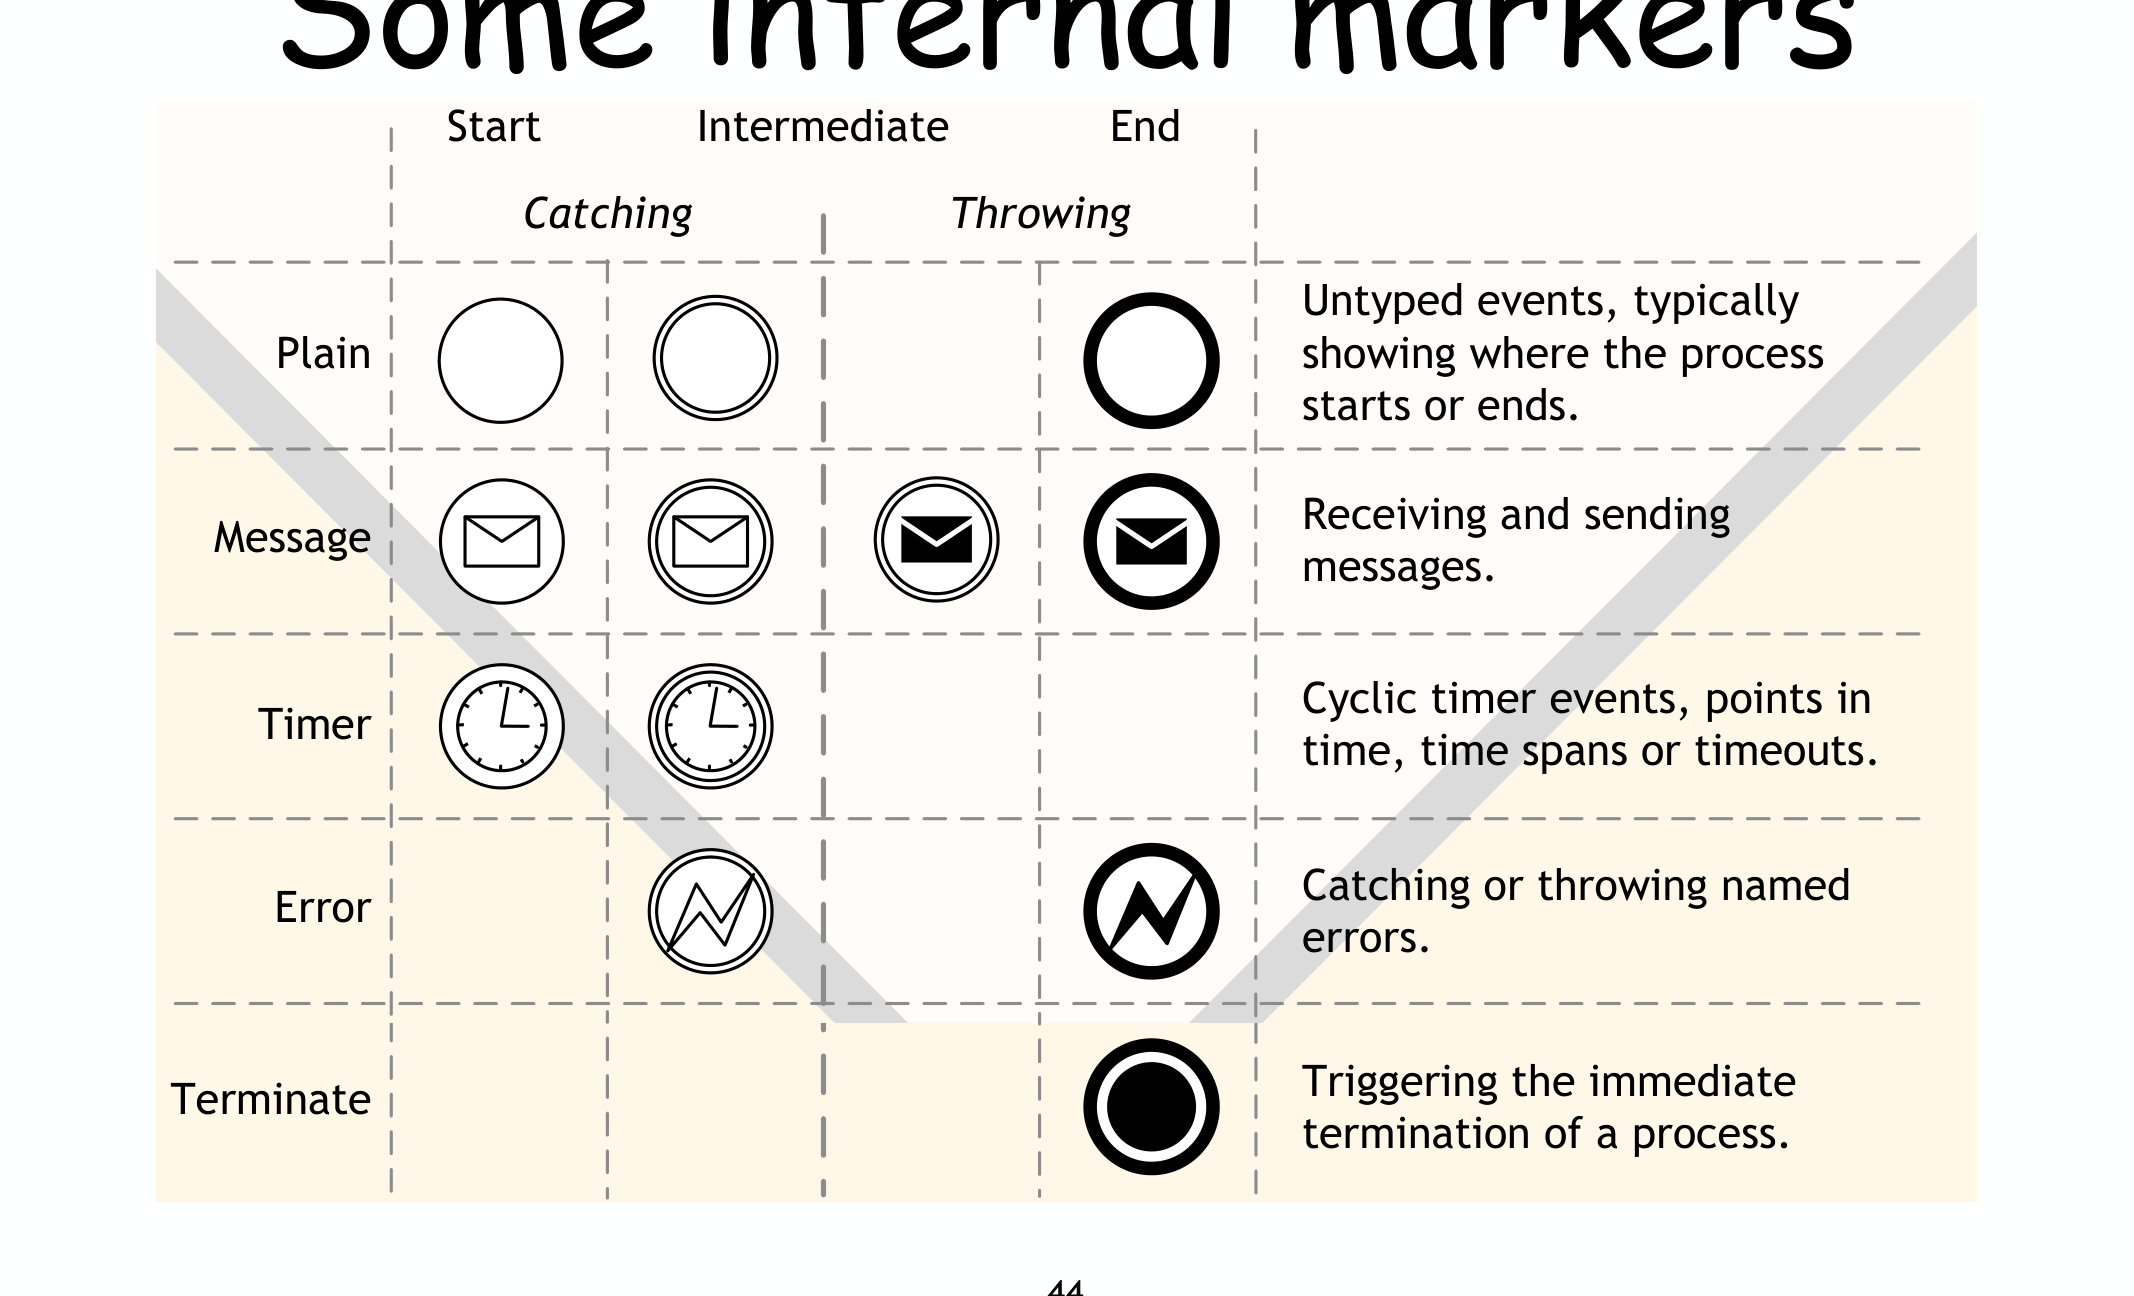
\includegraphics[width=0.74\linewidth,height=0.34\textheight,keepaspectratio]{images/07b-more-bpmn_p20_event-markers.png}
\caption{Alcuni marker interni degli eventi. La stessa forma-icona (busta, orologio, fulmine...) assume significato diverso a seconda che il bordo indichi start, intermediate o end, e a seconda che l'evento sia catching o throwing.}
\end{figure}

Alcuni casi tipici: un \textbf{intermediate message event} (busta) segnala l'attesa/ricezione di un messaggio, creando un "process break" in cui il processo si ferma finché il messaggio non arriva; un \textbf{timer start event} (orologio) crea un'istanza quando accade un certo evento temporale, mentre un \textbf{timer intermediate event} blocca il processo fino a un time-out; un \textbf{terminate end event} (cerchio pieno) causa la \textbf{cessazione immediata} dell'istanza corrente e di ogni sub-process (ma non del processo padre, se esiste).

\begin{boxnote}{Eventi vs attività}
BPMN non fa una distinzione netta, ma tipicamente: gli \textbf{eventi sono istantanei}, mentre le \textbf{attività hanno una durata}. Un messaggio ricevuto si può quindi modellare sia come \emph{receive task} (attività) sia come \emph{intermediate message event} (evento), a seconda che lo si voglia vedere come lavoro con durata o come istante.
\end{boxnote}

\section{\texorpdfstring{Collaboration e message flow}{Collaboration e message flow}}

Per modellare la comunicazione tra partecipanti si usa la \textbf{collaboration}, cioè un diagramma con \textbf{due o più pool}, ognuno un partecipante (che può essere collapsed o mostrare il processo interno). Ogni possibile comunicazione è un \textbf{message flow} tra pool.

\begin{boxdefinition}{Message flow}
Rappresenta una comunicazione (send/receive) tra \textbf{due partecipanti separati} (entità o ruoli di business), disegnato come una \textbf{linea tratteggiata con punta di freccia aperta} (e un pallino all'origine). Regole: ogni \textbf{evento} e ogni \textbf{attività} hanno \textbf{al più un} message flow; ogni \textbf{gateway} \textbf{nessuno} (i gateway non comunicano!); ogni \textbf{pool} un numero qualsiasi.
\end{boxdefinition}

Il passaggio da processo singolo a collaboration è graduale: si parte da un processo stand-alone, si aggiunge un pool collapsed che rappresenta il partner (black-box), poi lo si espande per mostrare l'interazione completa. I dati scambiati si possono annotare con i \textbf{message data object} (una busta che rappresenta il contenuto della comunicazione).

\begin{figure}[!htb]
\centering
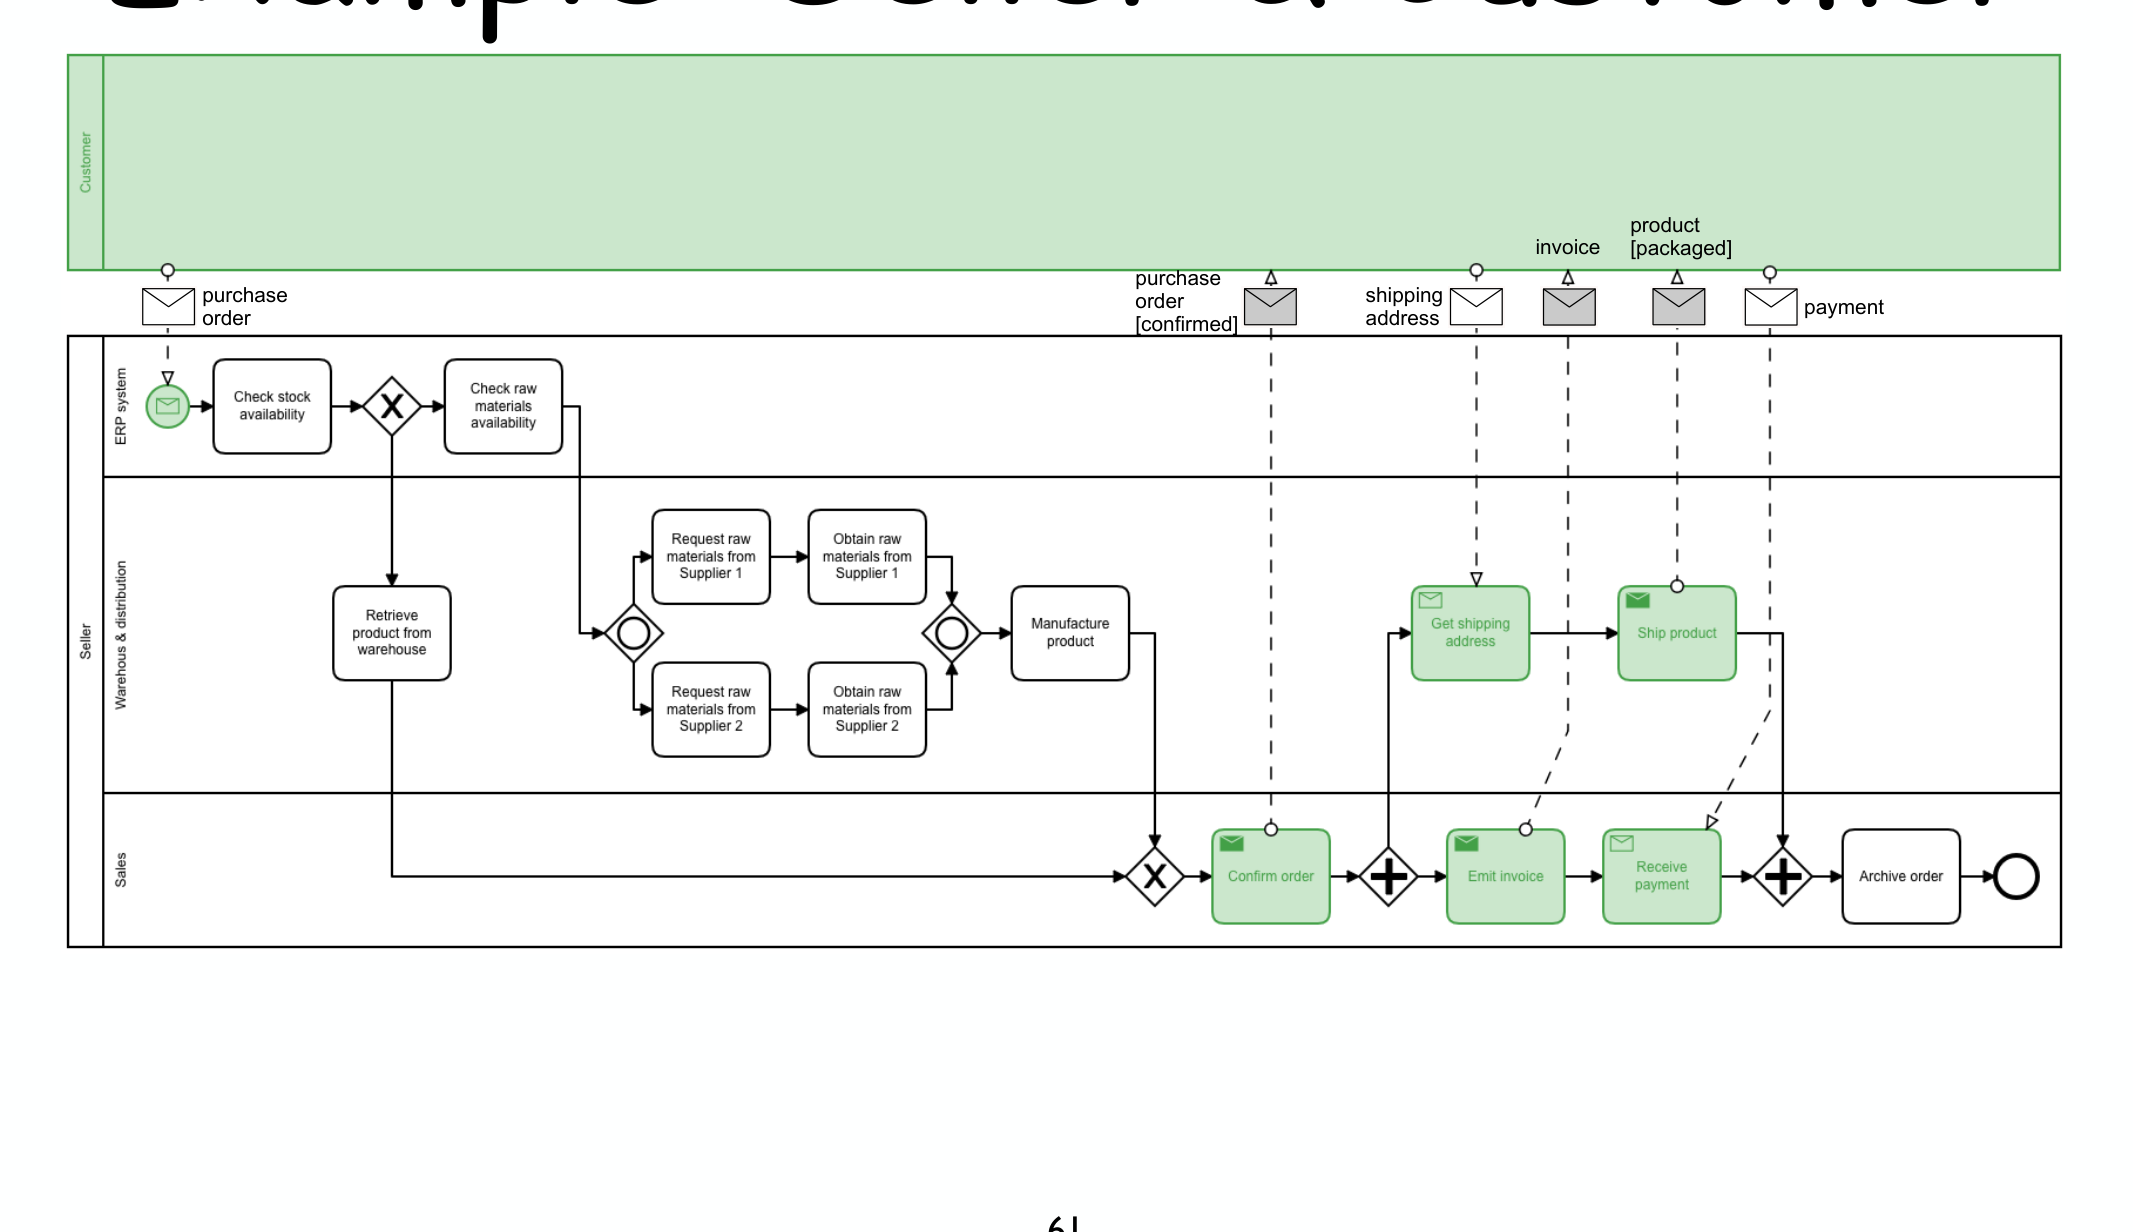
\includegraphics[width=0.74\linewidth,height=0.34\textheight,keepaspectratio]{images/07b-more-bpmn_p37_seller-customer.png}
\caption{Collaboration Seller \& Customer. Il pool del Seller è diviso in \textbf{lane} (ERP, Warehouse, Sales). Gli \textbf{oggetti-busta} sopra i message flow sono \textbf{message data object}: descrivono cosa viene scambiato (purchase order, invoice, payment, ...) e in quale stato (es. \texttt{[confirmed]}, \texttt{[packaged]}). I task verdi con l'icona busta sono attività di invio/ricezione messaggio.}
\end{figure}

\subsection{\texorpdfstring{Deferred choice: l'event-based gateway}{Deferred choice: l'event-based gateway}}

Un caso importante di comunicazione è la scelta che dipende da un \textbf{evento esterno}: non è il processo a decidere, ma "vince" ciò che arriva per primo. Per modellarlo BPMN ha l'\textbf{event-based (exclusive) gateway}, che è sempre seguito da eventi catching o receive task, e instrada il flusso verso l'evento/task che \textbf{accade per primo}. È esattamente la \textbf{scelta implicita / deferred} vista nei \hyperref[ch:04]{Petri net}: la decisione è rimandata al momento in cui uno degli eventi si verifica.

\section{\texorpdfstring{Data object, data store, associazioni}{Data object, data store, associazioni}}

Il \textbf{data object} (icona a documento con angolo piegato) rappresenta informazione che scorre nel processo — documenti, email, lettere. È un artefact: non influenza direttamente il flusso, ma dice \emph{quali informazioni} un'attività richiede o produce. Il suo \textbf{stato} si annota tra parentesi quadre (es. \texttt{Purchase order [confirmed]}). Per comodità lo \textbf{stesso} data object può comparire più volte nel diagramma, anche in stati diversi.

Il verso dell'\textbf{association} che lega data object e attività ne precisa il ruolo:

\begin{figure}[!htb]
\centering
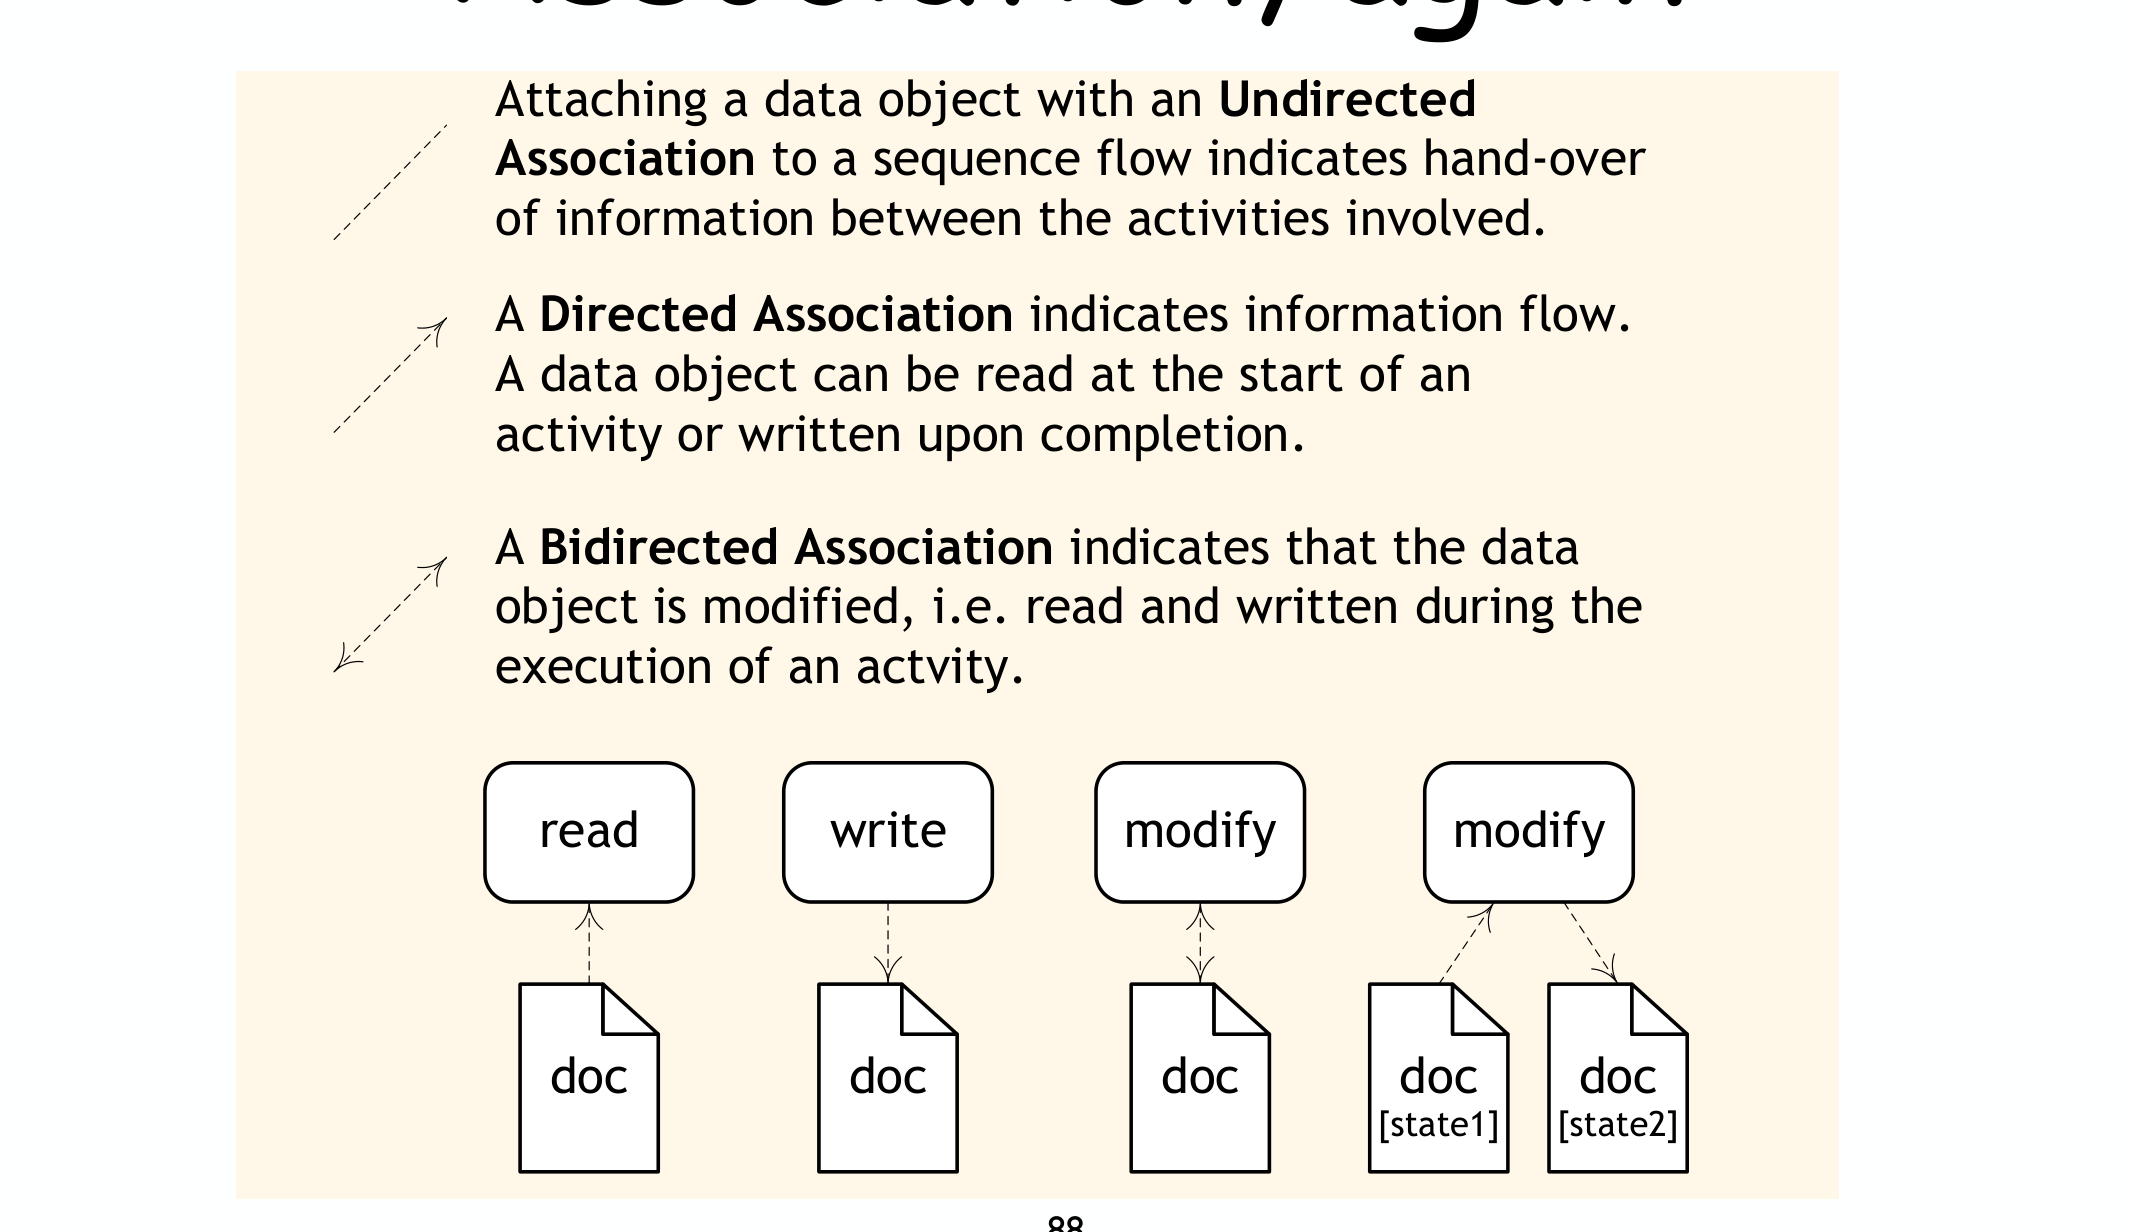
\includegraphics[width=0.74\linewidth,height=0.34\textheight,keepaspectratio]{images/07b-more-bpmn_p54_data-association.png}
\caption{Le associazioni dei data object. \textbf{Undirected} = passaggio di consegne; \textbf{Directed} = flusso informativo (read all'inizio / write alla fine); \textbf{Bidirected} = modifica (read e write durante l'esecuzione, es. da \texttt{[state1]} a \texttt{[state2]}).}
\end{figure}

Due varianti utili: il \textbf{data store} (persistente: un database o archivio che sopravvive oltre la vita dell'istanza di processo) e il \textbf{collection data object} (una collezione, es. la lista degli item di un ordine). Attenzione però: gli artefact danno informazione in più, ma \textbf{troppi artefact compromettono la leggibilità} del diagramma.

\section{\texorpdfstring{Call activity: riuso e sotto-processi globali}{Call activity: riuso e sotto-processi globali}}

Quando lo stesso sotto-processo serve in più modelli (per esempio un "Sign loan" usato sia per i mutui casa sia per i prestiti studenti), conviene definirlo \textbf{una volta sola} come processo globale e richiamarlo.

\begin{boxdefinition}{Call activity}
Un contenitore (wrapper) che \textbf{richiama} un sub-process o un task \textbf{definito globalmente}, riusandolo nel processo corrente. Si disegna con un \textbf{bordo spesso} per distinguerla da un sub-process locale.
\end{boxdefinition}

\begin{boxtip}{Vantaggi dei processi globali}
\begin{itemize}
\item \textbf{Readability}: i processi restano più piccoli, i dettagli sono altrove.
\item \textbf{Reusability}: si definisce una volta, si usa molte volte.
\item \textbf{Sharing}: ogni modifica al processo globale si \textbf{propaga automaticamente} a tutti i modelli che lo invocano.
\end{itemize}
\end{boxtip}

\subsection{\texorpdfstring{Attached (boundary) event: gestire eccezioni}{Attached (boundary) event: gestire eccezioni}}

Un evento intermedio può essere \textbf{attaccato al bordo} di un'attività: quando l'evento viene catturato, l'attività è \textbf{abortita} e il flusso prosegue lungo un ramo alternativo. È il meccanismo standard per la \textbf{gestione delle eccezioni}: un \textbf{error event} (icona a fulmine) attaccato a un'attività cattura un fault e attiva il recupero (es. il "redo" nell'esempio di image manipulation); una versione \emph{throwing} del fulmine lancia invece un'eccezione (es. un out-of-stock).

\section{\texorpdfstring{Choreography: la notazione a bande}{Choreography: la notazione a bande}}

Chiudiamo con le \textbf{choreography}, introdotte in BPMN 2.0 e già incontrate concettualmente in \hyperref[ch:06]{06 — Orchestration e Collaboration}. La differenza chiave con collaboration e orchestration è dove "vivono".

\begin{boxdefinition}{Choreography}
Definisce la \textbf{sequenza delle interazioni} tra partecipanti. A differenza degli altri diagrammi, \textbf{non esiste dentro un pool} e \textbf{non è eseguibile}: descrive solo come i partecipanti \emph{dovrebbero} comportarsi. Può usare i message data object.
\end{boxdefinition}

L'elemento base è il \textbf{choreography task}, che ha una notazione peculiare a \textbf{bande}.

\begin{figure}[!htb]
\centering
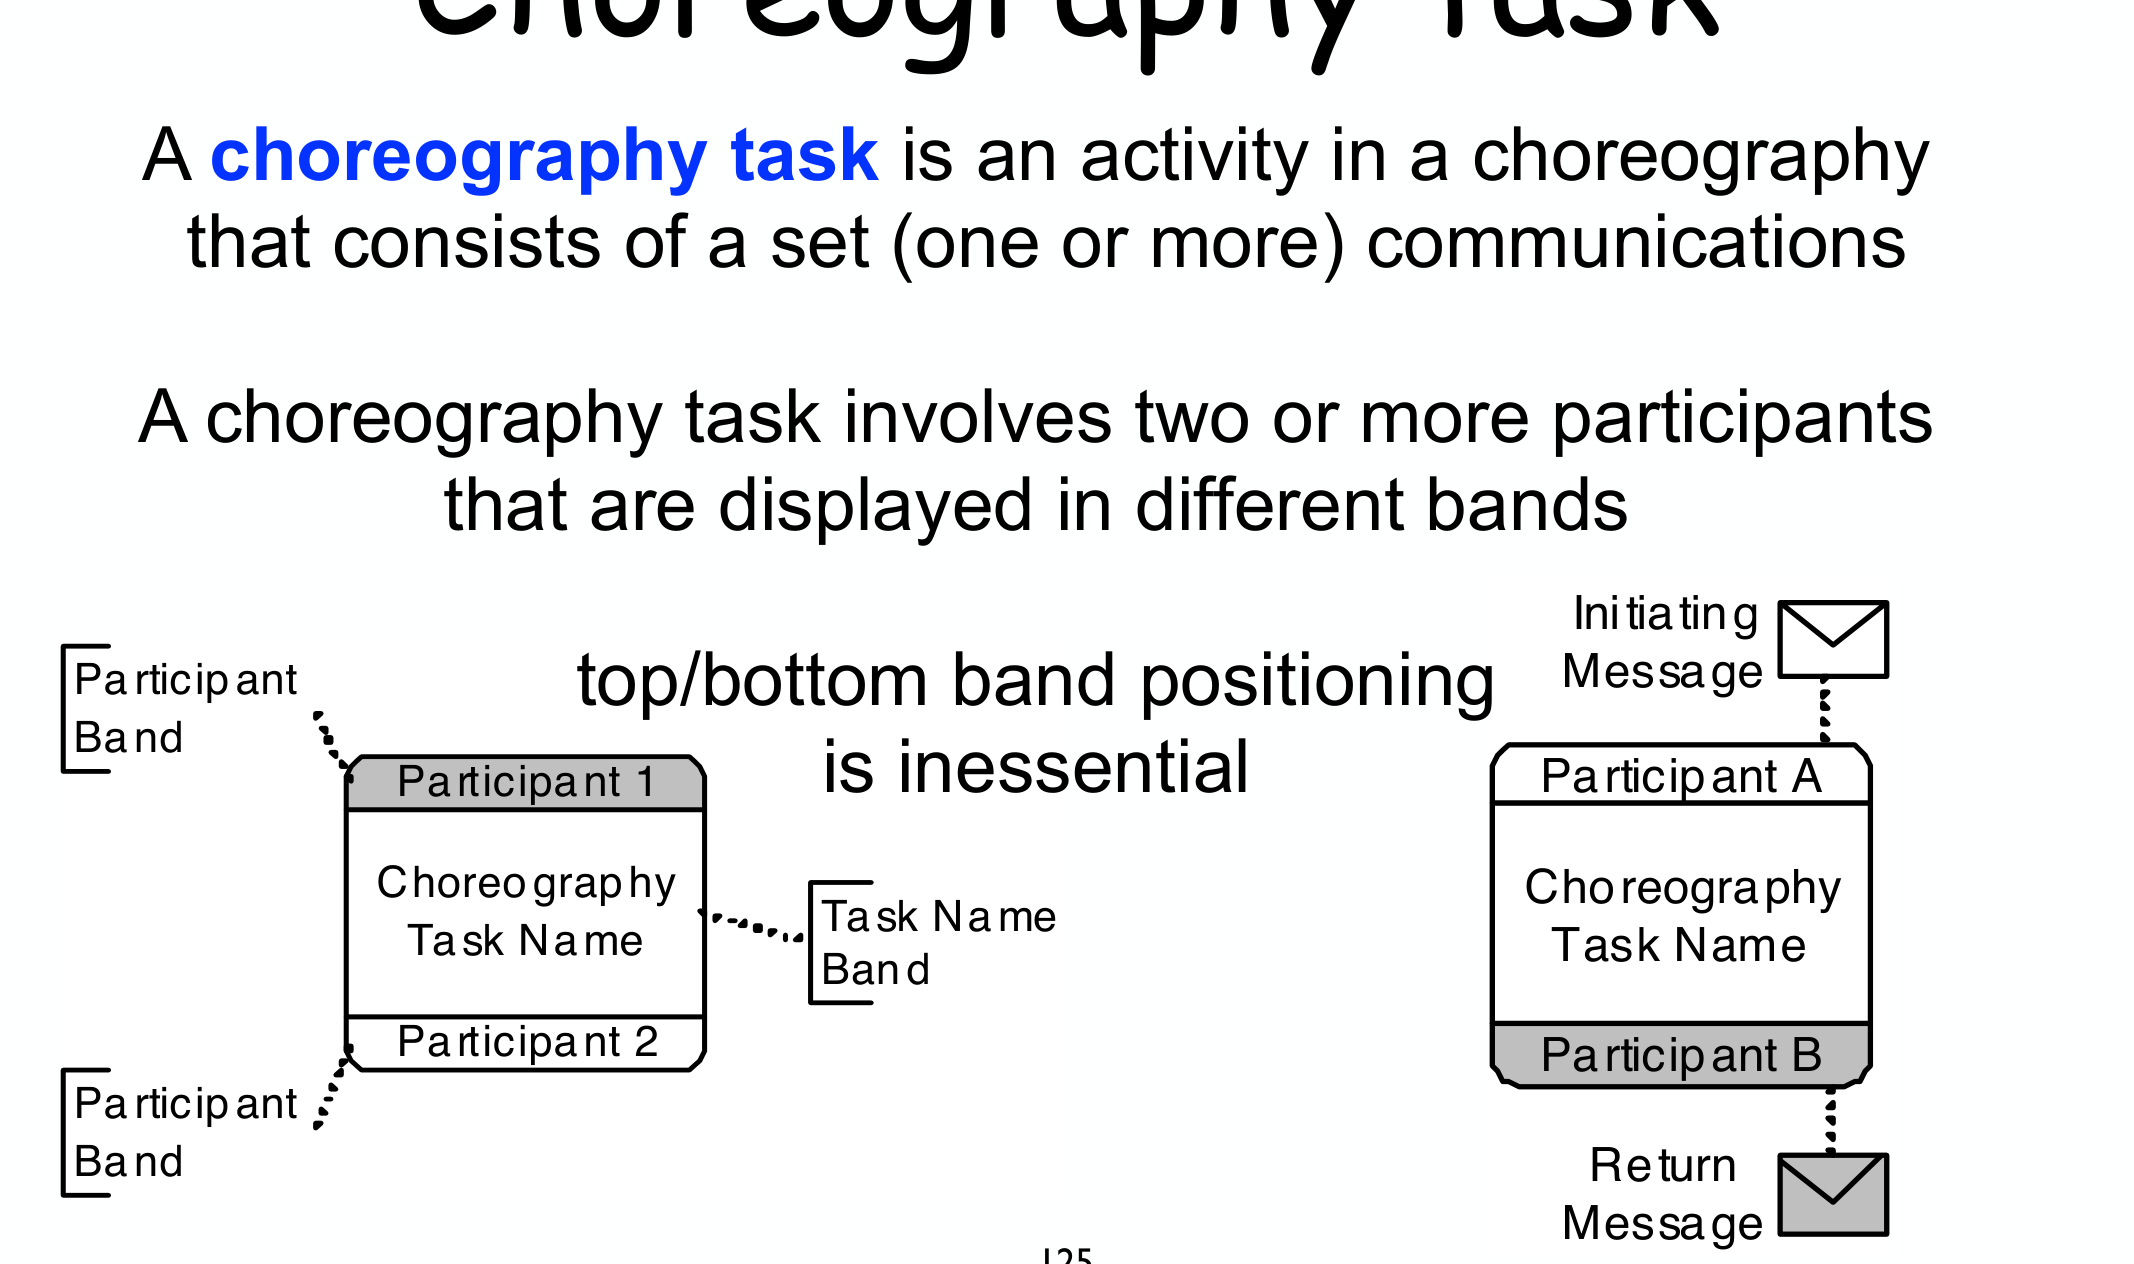
\includegraphics[width=0.74\linewidth,height=0.34\textheight,keepaspectratio]{images/07b-more-bpmn_p87_choreography-task.png}
\caption{Choreography task. Ogni banda (in alto/in basso, indifferentemente) è un \textbf{partecipante}; il centro è il nome del task, cioè l'interazione. Le buste rappresentano l'\textbf{Initiating Message} (chi avvia) e l'eventuale \textbf{Return Message} (la risposta).}
\end{figure}

Il flusso tra choreography task usa \textbf{sequence flow e gateway ordinari} per definire l'ordine delle interazioni; un vincolo importante è che \textbf{l'iniziatore di un'interazione deve aver partecipato a quella precedente} (altrimenti non saprebbe che è il suo turno).

\begin{boxnote}{Da collaboration a choreography e ritorno}
Le due viste sono collegate. Da una \textbf{collaboration} si ricava la choreography per \textbf{proiezione} su ciascun partecipante (si tiene solo la sua parte di interazioni). Viceversa, da una choreography si possono derivare i processi dei singoli partecipanti — ma non sempre il risultato è quello atteso: la \textbf{realizzabilità} di una choreography (esistono processi locali che, interagendo, riproducono esattamente la choreography globale?) è un problema non banale, collegato alla compatibilità vista in \hyperref[ch:06]{06 — Orchestration e Collaboration}.
\end{boxnote}

Con questo si chiude il quadro delle notazioni high-level. Da qui in avanti il corso torna ai \textbf{modelli formali} per \emph{analizzare} i processi, non solo descriverli. $\rightarrow$ \hyperref[ch:08]{08 — Nets Intro}